\documentclass{article}

%\usepackage{pdfpages}

\usepackage[utf8]{inputenc}

\begin{titlepage}


\title{Remote PC controller}
\author{Anindya Sundor Paul \\ Mehedi Hasan \\ S. M. Ariful Hoque \\ Fahad Chowdhury \\ Arafat Ahmed}
\date{ }

\begin{document}
 
\pagenumbering{gobble}

\maketitle
\end{titlepage}
 
\tableofcontents

\newpage

\pagenumbering{arabic}
 
\section{Introduction}

The project we will be working on is remote PC controller. The main idea of this project is to control a computer remotely by another computer. The computers will be connected through LAN. We have to send signals to control the functions of mouse and keyboard. \\

\section{Motivation}

The concept of this project comes from the idea of solving a computer's problem remotely. It is an interesting project to work on as numerous new features have to be worked upon. Through this project we will get a clear concept about different networking protocol and network programming. %modification needed
Similar programs are available (i.e. TeamViewer).

%Can add another section called project summary

\section{Project Details}

In this section we will be discussing the detailed functions of this project and how we will implement these functions.

\subsection{Members of the Team}

Our team consists of five members.\\ \\
\textbf{Anindya Sundor Paul} : CEO.\\
\textbf{S. M. Ariful Hoque} : Backend developer.\\
\textbf{Fahad Chowdhury Sabah} : Frontend developer.\\
\textbf{Mehedi Hasan} : Frontend developer.\\
\textbf{Arafat Ahmed Tanim} : Frontend developer.\\ \\
\textbf{Anindya Sundor Paul} will organize and supervise our project. He will also work as a backend developer. He will generate the basic algorithm to complete the project. The design of the UI is also done by him.\\ \\
\textbf{S. M. Ariful Hoque} will work as a backend developer. He will do the core programming of the project. Based on Anindya Sundor Paul's algorithm, he will develop the system.\\ \\
\textbf{Fahad Chowdhury Sabah}, \textbf{Mehedi Hasan} and \textbf{Arafat Ahmed Tanim} will work as frontend developer. Based on the design, they will create the UI. Creating different buttons and make them functinal is their prime job. They will use different library (i.e. Java Swing).\\ \\
Although the job is divided among all the members of the team, it is very much possible for one member to participate in another one's job.

\subsection{Design} The basic algorithm is given by Anindya Sundor Paul. The primary UI design is also done by him although it is modifiable. 

\subsubsection{Workflow Diagram}

This is the workflow diagram of our project.\\ \\
%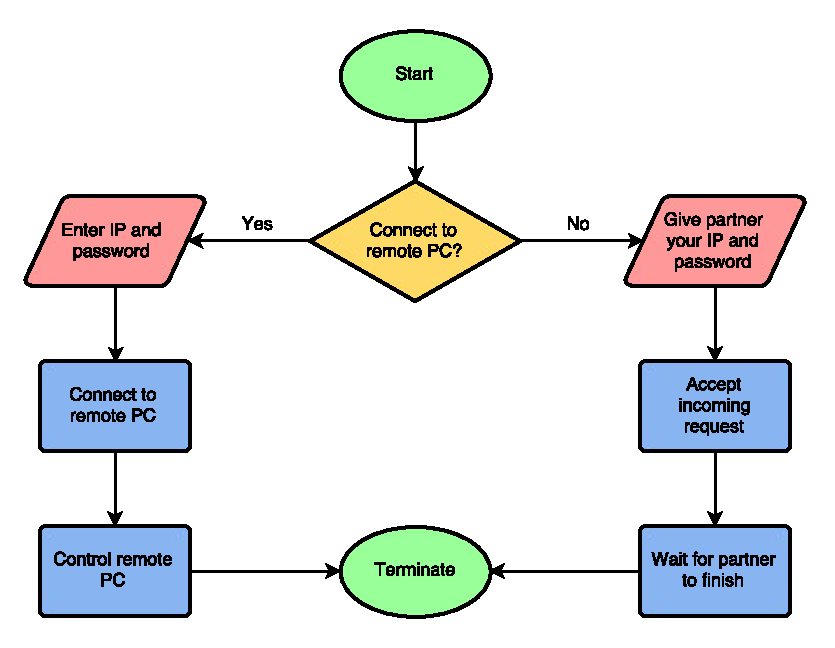
\includepdf[pages=-]{remote-pc-controller-workflow.pdf}
%here goes the pdf
After starting the program, the user may act as controlled or controller. If the user wants to connect to remote PC and control it, he/she has to enter the IP and password provided by the remote PC. After entering valid IP and password the controller will send a request in order to have control. After accepting the request, the controller will have control of the remote PC. The remote PC user will also have access to his computer and may terminate at any point. After connecting to the remote PC, the controller will do his job and then terminate the program. \\
If the user wants his PC to be controlled, he/she will have to give his/her IP and password to the controller. This is a password generated for this sole program, not the master password. After getting the password and IP, the controller will send a request. If the remote PC user do not accept the request, the connection will not be made. If he/she accepts it, the controller will have control over the remote PC. The remote PC user may terminate the program at any moment.\\

\subsubsection{User Interface}

We have tried our best to come up with a UI design so that the user can use the program very easily. Here is the design.\\ \\ 
%Goes the pdf
%Allow remote control
This window will appear at the start of the program. The Allow Remote Control part of the window will show the host PC, its IP address and a randomly generated password. If the user likes to allow remote control, he/she will provide these information to the controller. \\
Control Remote PC part of the window will contain two dialog boxes to put the partner's IP and password. The controller will put the informations and send a request. If the remote PC user accepts the requests, then the connection will be built. 
%Incoming request
This window will show up if any computer is trying to connect to a remote PC. This window shows the IP address of the requester. If the user of the remote PC allows the request, the requester will have control over the remote PC. \\
%current Session
This window will appear during a session. This window will only show the controller's IP address. The contolled PC user may terminate the connection at any point using Disconnect button. \\
%Oops
This is a warning message. If the inserted IP and password do no match, then this window will appear.
%connecting
This window will show up while the two PCs are connecting.
%Denied
If the remote PC user does not want the connection to be built, he/she can deny the request. In this case this window will appear.

%\subsection{Use Case Diagram} if possible

\section{Our Goal}
Our main goal is to complete the basic project, which is to control a PC remotely through LAN by another PC. If it is completed before estimated time, we will try to implement some extensions.


\section{Conclusion}
Remote-PC-controller is a basic network programming project. This project will help us to have a better and clearer concept about different networking protocol and file transferring. Our goal is to complete this project within the fastest time and without any bug.

\end{document}